\documentclass[a4paper]{article}
\usepackage[margin=2cm]{geometry}

\RequirePackage{luatex85}
\def\pgfsysdriver{pgfsys-pdftex.def}

\usepackage{fontspec}
\usepackage[english]{babel} % Language 
\usepackage{enumitem}
\usepackage{listings}
\usepackage[dvipsnames]{xcolor}
\usepackage{graphicx}
\usepackage{float}
\usepackage[hidelinks]{hyperref}
\usepackage{tikz}
\usepackage{pgfplots}

\pgfplotsset{compat=1.14}

\setlength{\parindent}{0pt}
\setlength{\parskip}{1em}

\lstset{
    basicstyle=\ttfamily\footnotesize,
    keywordstyle=\color{blue},      % keyword style
    commentstyle=\color{OliveGreen},   % comment style
    stringstyle=\color{purple}, 
    tabsize=4,
    frame=single,
    numbers=left,                   % where to put the line-numbers
    numberstyle=\tiny\color{gray},  % the style that is used for the line-numbers
}

\title{
	\textsc{PAR: Laboratory 1} \\
	\texttt{\large par4201}
	}
	
\author{Joan Marcè i Igual \and Esteve Tarragó i Sanchís}

\begin{document}

\maketitle

\section*{Node architecture and memory}

\begin{enumerate}
	\item \textbf{Draw and briefly describe the architecture of the computer in which you are doing this lab session (number of sockets, cores per socket, threads per core, cache hierarchy size and sharing and amount of main memory).}
\end{enumerate}

\begin{itemize}
	\item Processor
	\begin{itemize}
		\item Number of sockets: 2
		\item Cores per socket: 6
		\item Threads per core: 2
	\end{itemize}
	
	\item Cache
	\begin{itemize}
		\item L1 instructions cache (32KB) not shared
		\item L1 data cache (32KB) not shared
		\item L2 cache (256KB) not shared
		\item L3 cache (12MB) shared
	\end{itemize}
	
	\item Memory
	\begin{itemize}
		\item Main memory: 23GB
		\item NUMA node memory: 12 GB
	\end{itemize}
\end{itemize}

\section*{Timing sequential and parallel executions}

\begin{enumerate}[resume]
	\item \textbf{Describe what do you need to add to your program to measure elapsed execution time between a pair of points in the program, clearly indicating the library header file that needs to be included, the library functions that need to be invoked and the data structure and its fields.}
\end{enumerate}

You need to call the \texttt{gettimeofday()} function when you want to start measuring the time and the same function again when you want to stop. 

\begin{lstlisting}[language=C]
    #include <time.h>

    gettimeofday(struct timeval *tv, struct timezone *tz);
    
    struct timeval {
        time_t       tv_sec;    // seconds
        susseconds_t tv_usec;   // microseconds since the Epoch
    }
    
    struct timezone {
        int tz_minteswest;      // minutes west of Greenwich
        int tz_dsttime;	        // type of DST correction
    }
\end{lstlisting}

The \texttt{gettimeofday()} function returns the seconds and microseconds since January the 1st, 1970. Then you can subtract the final microseconds with the starting microseconds to know the function's elapsed time. 

\begin{enumerate}[resume]
	\item \textbf{Plot the speed-up obtained when varying the number of threads (strong scalability) and problem size (weak scalability) for \texttt{pi\_omp.c}. Reason about how the scalability of the program.}
\end{enumerate}

\begin{figure}[H]
    \begin{minipage}[t]{0.5\linewidth}
        \begin{tikzpicture}
            \begin{axis}[
                    xlabel = Threads,
                    ylabel = Speed-up,
                    xmin = 0, xmax = 13,
                ]
                \addplot table[x=Threads,y=Speedup, col sep = semicolon] {speedup_strong.dat};
                \addplot+ [mark=none, dashed, domain = {1:12}] {x};
            \end{axis}
        \end{tikzpicture}
        \caption{Speedup strong}
        \label{fig:speedup_strong}
    \end{minipage}
    \begin{minipage}[t]{0.5\linewidth}
        \begin{tikzpicture}
            \begin{axis}[
                    xlabel = Threads,
                    ylabel = Speed-up,
                    xmin = 0, xmax = 13,
                    ymin = 0, ymax = 1.1,
                ]
                \addplot table[x=Threads,y=Speedup, col sep = semicolon]{speedup_weak.dat};
                \addplot+ [mark=none, dashed, domain ={1:12}]{1};
            \end{axis}
        \end{tikzpicture}
        \caption{Speedup weak}
        \label{fig:speedup_weak}
    \end{minipage}
\end{figure}

\begin{figure}[H]
    \begin{minipage}[t]{0.49\linewidth}
        \begin{tikzpicture}
            \begin{axis}[
                    xlabel = Threads,
                    ylabel = Speed-up,
                    xmin = 0, xmax = 13,
                ]
                \addplot table[x=Threads,y=Time, col sep = semicolon] {time_strong.dat};
            \end{axis}
        \end{tikzpicture}
        \caption{Time strong}
        \label{fig:time_strong}
    \end{minipage}
    \begin{minipage}[t]{0.49\linewidth}
        \begin{tikzpicture}
            \begin{axis}[
                    xlabel = Threads,
                    ylabel = Speed-up,
                    xmin = 0, xmax = 13,
                ]
                \addplot table[x=Threads,y=Time, col sep = semicolon]{time_weak.dat};
            \end{axis}
        \end{tikzpicture}
        \caption{Time weak}
        \label{fig:time_weak}
    \end{minipage}
\end{figure}


As it can be seen in the graphics there's always an overhead for creating and destroying the threads. Ideally the speedup in the \autoref{fig:speedup_strong} should be $y = x$ but instead there is not. Moreover, this is more obvious in the \autoref{fig:speedup_weak} the speedup should be $1$ but it decreases as the number of threads increase.

\section*{Visualizing the task graph and data dependences}

\begin{enumerate}[resume]
	\item \textbf{Include the source code for function \texttt{dot\_product} in which you show the \textit{Tareador} instrumentation that has been added to study the potential parallelism in the code. This instrumentation has to appropriately define tasks and filter the analysis of variable(s) that cause dependence(s).}
\end{enumerate}
% {6,9,25,27,29,31,35,37}
\lstinputlisting[language=C, title=\lstname]{dot_product.c}

Thanks to \texttt{Tareador} we could see there was a strong dependency caused by the variable \texttt{result}. That’s why we disable it for the analysis.

\begin{enumerate}[resume]
	\item \textbf{Capture the task dependence graph for that task decomposition and the execution timelines (for 8 processors) that allow you to understand the potential parallelism attainable. Briefly comment the relevant information that is reported by the tools.}
\end{enumerate}

\begin{figure}[H]
    \centering
    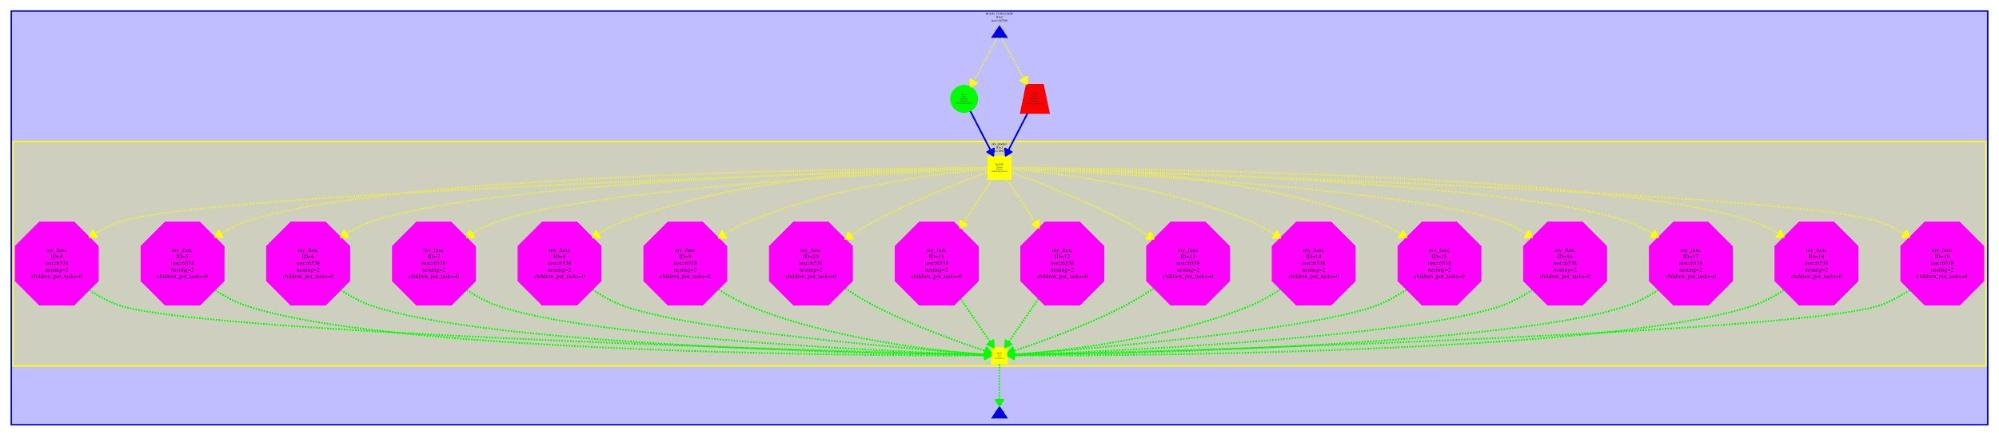
\includegraphics[width=\textwidth]{image03}
    \caption{Tareador nodes}
    \label{fig:tareador_nodes}
\end{figure}
\begin{figure}[H]
    \centering
    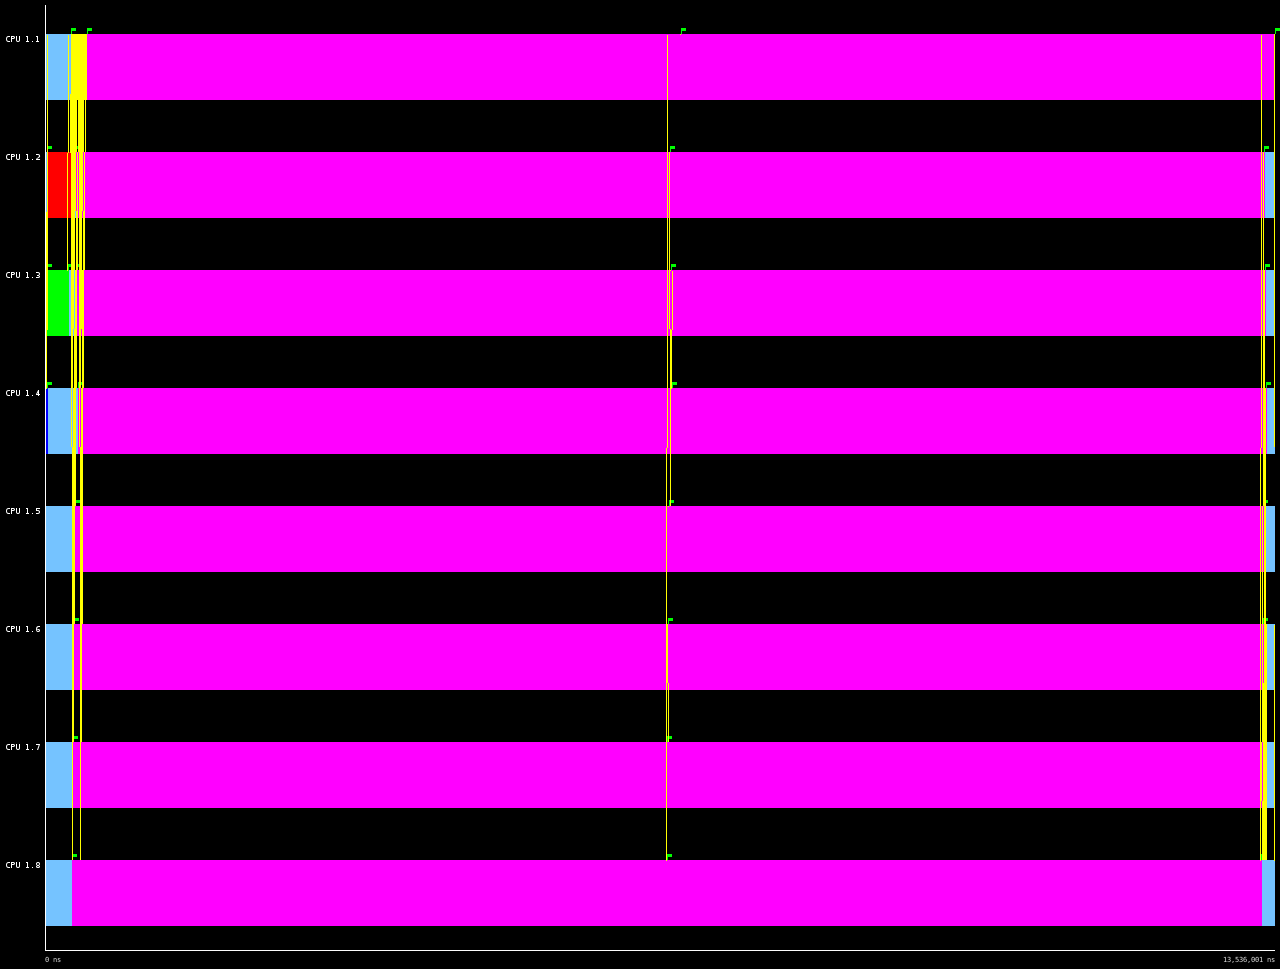
\includegraphics[width=\textwidth]{image02}
    \caption{Tareador execution timeline}
    \label{fig:tareador_timeline}
\end{figure}

This tool allow us to calculate the critical path of a parallel program given a task decomposition. It also helps us to see dependencies between task so we can reduce them by protecting variables.

It’s also useful if we want to anticipate what will be our speed up with N processors because we can see which task will be assigned to each processor and when will all the processors finish.

\section*{Analysis of task decompositions}

\begin{enumerate}[resume]
	\item \textbf{Complete the following table for the initial and different versions generated for \texttt{3dfft\_seq}, briefly commenting the evolution of the metrics with the different versions.}
\end{enumerate}

\begin{center}
	\begin{tabular}{l|rrr}
		Version & $T_1(ms)$ & $T_{\infty}(ms)$ & Parallelism \\
		\hline
		seq & 593 & 593 & 1 \\
		v1 & 593 & 593 & 1 \\
		v2 & 593 & 315 & 1,88 \\
		v3 & 593 & 108 & 5,49 \\
		v4 & 593 & 59 & 10
	\end{tabular}
\end{center}

\begin{enumerate}[resume]
	\item \textbf{With the results from parallel simulation with 2, 4, 8, 16 and 32 processors, draw the execution time and speedup plots for version v4 with respect to the sequential execution (that you can estimate from the simulation of the initial task decomposition that we provided in \texttt{3dfft\_seq.c}, using just 1 processor). Briefly comment the scalability behavior shown on these two plots.}
\end{enumerate}

\begin{center}
    \begin{tabular}{l|rrrrr}
        Processors & 2 & 4 & 8 & 16 & 32 \\
        \hline
        Time (ms) & 297 & 156 & 87 & 59 & 59
    \end{tabular}
\end{center}

\begin{figure}[H]
    \centering
    \begin{tikzpicture}
        \begin{semilogxaxis}[
                xlabel = { Processors },
                ylabel = { Time (ms) },
                xmin = 0, xmax = 34,
                ymin = 0, ymax = 310,
                xtick = {2, 4, 8, 16, 32},
                log ticks with fixed point
            ]
            \addplot[color=blue,mark=*] coordinates {
                (2,297)(4,156)(8, 87)(16,59)(32,59)
            };
        \end{semilogxaxis}
    \end{tikzpicture}
\end{figure}

\section*{Tracing sequential and parallel execution}

\begin{enumerate}[resume]
	\item \textbf{From the instrumented version of \texttt{pi\_seq.c}, and using the appropriate \texttt{Paraver} configuration file, obtain the value \textit{parallel fraction} $\phi$ for this program when executed with 100.000.000 iterations, showing the steps you followed to obtain it.}
\end{enumerate}

We executed the program in a separate node with \verb|> qsub -l execution ./submit-seq-i.sh| and then we obtained the \verb|.prv| file that we opened with Paraver. Then we were able to obtain the execution times.

$$
\phi = \frac{parallel}{parallel + serial} = \frac{788398}{21417,136 + 788398,214} = 0,99997826526
$$

\begin{figure}[H]
    \centering
    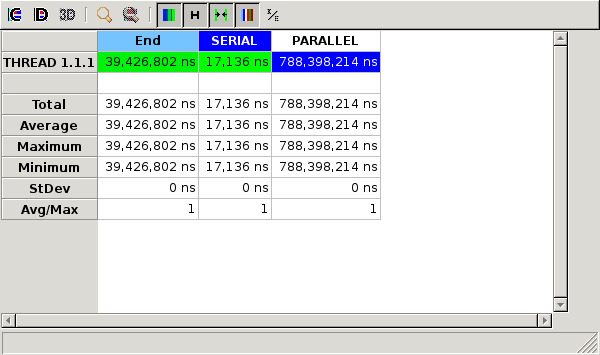
\includegraphics[width=\textwidth]{image01}
    \caption{Paraver statistics}
\end{figure}

\begin{enumerate}[resume]
	\item \textbf{From the instrumented version of \texttt{pi\_omp.c}, and using the appropriate \texttt{Paraver} configuration file, show a profile of the \% of time spent in the different OpenMP states when using 8 threads and for 100.000.000 iterations. Draw your own conclusions from that profile.}
\end{enumerate}

\begin{figure}[H]
    \centering
    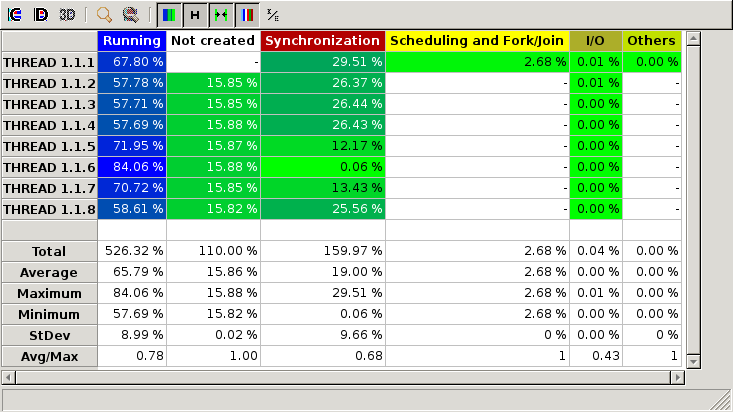
\includegraphics[width=\textwidth]{image04}
    \caption{Paraver omp statistics}
\end{figure}

\begin{itemize}
    \item Total running time: $526,32\%$
    \item Time not being created: $110\%$
    \item Time not synchronizing: $157,97\%$
    \item Time scheduling and fork/join: $2,68\%$
    \item I/O Time: $0,4\%$
\end{itemize}

\begin{itemize}
    \item Total running time: $196,721,828ns$
    \item Theoretical speedup: $ \frac{Serial + Parallel}{Serial + \frac{1}{8}Parallel} = 7,9988 $
    \item Real speedup: $\frac{Total serial}{Total Parallel} = 4.2082 $
\end{itemize}

As we can see the real speedup is less inferior than the theoretical speedup. This is due to the time lost in the synchronization and the fork/join process. The synchronization time takes about $159.97\%$ of CPU time which is about $19.996\%$ of the execution time.

\end{document}